% !TeX root = ../report.tex
\section{Introduction to reinforcement learning}
Reinforcement learning is a machine learning paradigm dedicated to solving sequential decision processes. The definition of a reinforcement learning algorithm given by \citet[chap. 3]{RLBook2018}, is an algorithm which can solve a specific kind of sequential decision problem, namely those which can be described formally by a \textit{finite Markov decision process}.


\subsection{Finite Markov Decision Processes}

The Markov decision process provides a formal description of sequential decision problems. 

In this project, we define a Markov decision process by a 4-tuple $(\mathcal{S},\mathcal{A},\mathcal{R}, p)$, where $\mathcal{S}$ is the finite state-space, $\mathcal{A}$ is the finite action-space, $\mathcal{R} \subset \mathbb{R}$ is the finite reward-space, and the dynamics function $p : \mathcal{S} \times \mathcal{R} \times \mathcal{S} \times \mathcal{A} \rightarrow [0,1]$, defined in \cref{eq:p_def}, describes the conditional probability of entering a state $s' \in \mathcal{S}$ with reward $r \in \mathcal{R}$ given the previous state was $s \in \mathcal{S}$ and action $a \in \mathcal{A}(s)$ was chosen.
\begin{align}
    \label{eq:p_def} p(s',r\ |\ s,a) \defeq \Pr{S_t\!=\!s', R_t\!=\!r\ |\ S_{t-1}\!=\!s, A_{t-1}\!=\!a}
\end{align}
Some like to include $\gamma$, a \textit{discount factor} in the definition of finite MDP. 
We, however, leave this definition to the individual reinforcement learning algorithm.


\vspace*{1em}

When solving Markov decision processes, a sequence of random variables is introduced. Let $T = \set{1, 2, \ldots}$ be a sequence of discrete time steps, $S_t$ is then a random variable which indicates the state of the environment at time step $t \in T$, $A_t$ is the action chosen at time step $t \in T$, from the set $\mathcal{A}(s)$ which denotes the actions available from state $s$. 
$R_t$ is the reward received after choosing action $A_{t-1}$ from state $S_{t-1}$

%\begin{align}
%    \sum_{s' \in \mycal{S}}\sum_{r \in \mycal{R}} p(s', r, s, a) &= 1 & \forall s \in \mycal{S}, \forall a \in \mycal{A}(s)\\
%    p(s'\ |\ s,a) \defeq \Pr{S_t=s'\ |\ S_{t-1} = s, A_{t-1} = a} &= \sum_{r\in \mycal{R}}p(s',r\ |\ s,a) & \forall s,s' \in \mycal{S}, \forall a \in \mycal{A}(s)\\
%    \Ex{R_t\ |\ S_{t-1}=s, A_{t-1}=a} &= \sum_{r \in \mycal{R}} r \sum_{s' \in \mycal{S}} p(s', r\ |\ s, a) & \forall s \in \mycal{S}, \forall a \in \mycal{A}(s)\\
%    \Ex{R_t\ |\ S_{t-1}=s, A_{t-1}=a, S_t=s'} &= \sum_{r \in \mycal{R}} r \frac{p(s', r\ |\ s, a)}{p(s'\ |\ s, a)} & \forall s,s' \in \mycal{S}, \forall a \in \mycal{A}(s)
%\end{align}
%\replace{Text for above}

\vspace*{1em}

\Cref{fig:agent-environment} visualises the agent-environment loop. 
Initially, the agent is placed in some environment \mycal{E}, from where the agent observes $S_0$.
The agent the chooses some action $A_0 \in \mycal{A}(S_0)$, after the action has been performed, state $S_{t+1}$ and $R_t$ is presented to the agent, this results in a sequence of the form $S_0,A_0,R_1,S_1,A_1,R_2,S_2,\ldots$

\begin{figure}[!htb]
    \centering
    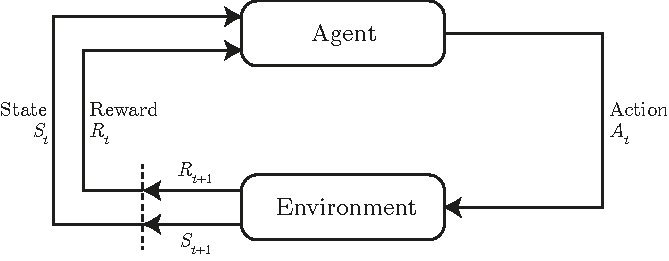
\includegraphics[scale=1]{../include/agent-environment-loop.pdf}
    \caption{The Agent-Environment interface adapted from \citet[chap. 3]{RLBook2018}}
    \label{fig:agent-environment}
\end{figure}

As such, the agent will learn the optimal \textit{policy} $\pi^*$ (or estimate thereof) by iteratively taking actions, and observing the following reward, and state of the environment.



\begin{figure}[!htb]
    \centering
    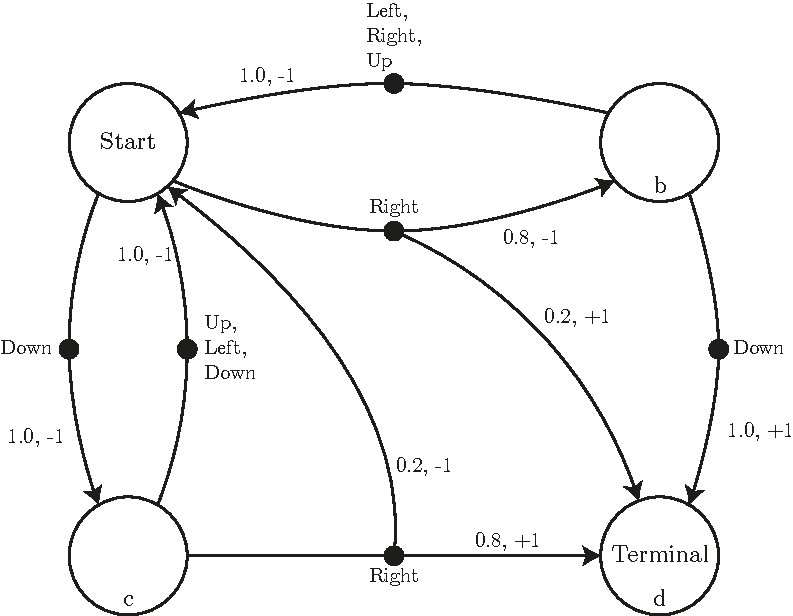
\includegraphics[scale=0.8]{../include/PDF/MDP.pdf}
    \caption{\todo}
    \label{fig:MDP}
\end{figure}

\begin{figure}[!htb]
    \centering
    \replace{Visual MDP representation for small example?}
    \caption{MDP represented as a graph}
    \label{fig:mdp-graph-repr}
\end{figure}

\subsection{RL}
according to some policy $\pi$ either \textit{exploitatively} or \textit{exploratively}.
